\usetikzlibrary{shapes,arrows,positioning,calc}

\tikzset{
    block/.style = {draw, fill=white, rectangle, minimum height=3em, minimum width=3em},
    tmp/.style  = {coordinate},
    sum/.style= {draw, fill=white, circle, node distance=1cm},
    input/.style = {coordinate},
    output/.style= {coordinate},
    pinstyle/.style = {pin edge={to-,thin,black}
        }
}


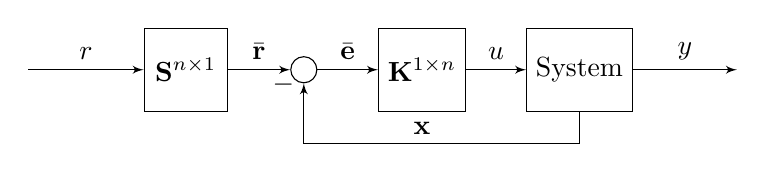
\begin{tikzpicture}[auto, node distance=2cm,>=latex']
    \node [input, name=rinput, node distance=1.5cm]         (rinput)        {};
    \node [block, right of=rinput]                          (scale_vec)     {$\mathbf{S}^{n\times 1}$};
    \node [sum, right of=scale_vec, node distance=1.5cm]    (sum1)          {};
    \node [block, right of=sum1, node distance=1.5cm]       (static_gain)   {$\mathbf{K}^{1\times n}$};
    \node [tmp, below = 0.4cm of static_gain]               (tmp1)          {$\mathbf{x}$};
    \node [block, right of=static_gain]                     (sys)           {System};
    % \node [output, below of=sys] (x) {};
    \node [output, right of=sys, node distance=2cm] (output) {};
    \node at (5,-.75) {$\mathbf{x}$} ;

    \draw [->] (rinput) -- node{$r$} (scale_vec);
    \draw [->] (scale_vec) -- node{$\bar{\mathbf{r}}$} (sum1);
    \draw [->] (sum1) -- node{$\bar{\mathbf{e}}$} (static_gain);
    \draw [->] (static_gain) -- node{$u$} (sys);
    \draw [->] (sys) -- node{$y$} (output);
    \draw [->] (sys) |-(tmp1) -| node[pos=0.99] {$-$} (sum1);
\end{tikzpicture}